% NeurIPS poster: recall vs recognition memory in a small Gated DeltaNet-2.
% Numbers: reports/recall_vs_recognition.md (experiments 1-2) and results/sweep/summary.json (experiment 3, 84 runs).
% Build:  conda run -n ai python posters/make_poster_figures.py
%         cd posters && latexmk -pdf neurips_poster.tex   (or pdflatex twice)
\documentclass{article}
\usepackage[paperwidth=48in,paperheight=36in,margin=0.9in,top=0.7in,bottom=0.7in]{geometry}
\usepackage[T1]{fontenc}
\usepackage[sfdefault]{FiraSans}
\usepackage{anyfontsize}
\usepackage{graphicx,xcolor,tikz,tcolorbox,enumitem,booktabs,qrcode,amsmath,amssymb}
\usetikzlibrary{positioning,calc,arrows.meta,decorations.pathreplacing}
\tcbuselibrary{skins}
\graphicspath{{figures/}}
\pagestyle{empty}
\setlength{\parindent}{0pt}
\setlength{\parskip}{0.35em}

\definecolor{ink}{HTML}{1A1A1A}
\definecolor{ink2}{HTML}{52514E}
\definecolor{muted}{HTML}{8A8984}
\definecolor{rule}{HTML}{E6E5E0}
\definecolor{paper}{HTML}{FAFAF8}
\definecolor{navy}{HTML}{0D366B}
\definecolor{recall}{HTML}{2A78D6}
\definecolor{recog}{HTML}{EB6834}
\definecolor{curr}{HTML}{1BAF7A}
\definecolor{recallbg}{HTML}{EAF2FC}
\definecolor{recogbg}{HTML}{FDEDE5}

% body ~30pt; everything else relative to it
\renewcommand{\normalsize}{\fontsize{30}{39}\selectfont}
\renewcommand{\small}{\fontsize{25}{32}\selectfont}
\renewcommand{\footnotesize}{\fontsize{22}{28}\selectfont}
\renewcommand{\large}{\fontsize{36}{44}\selectfont}
\newcommand{\RC}[1]{\textcolor{recall}{\textbf{#1}}}
\newcommand{\RG}[1]{\textcolor{recog}{\textbf{#1}}}
\setlist{leftmargin=1.1em,itemsep=0.25em,topsep=0.2em,label=\textcolor{navy}{\textbullet}}

\newtcolorbox{block}[2][]{enhanced,colback=white,colframe=rule,boxrule=2pt,arc=10pt,
  left=0.45in,right=0.45in,top=0.35in,bottom=0.35in,before skip=0pt,after skip=0.55in,
  title={\fontsize{44}{52}\selectfont\bfseries #2},coltitle=navy,colbacktitle=white,
  attach title to upper,after title={\par\vspace{0.25in}},#1}
\newtcolorbox{keybox}[1][]{enhanced,colback=navy,colframe=navy,coltext=white,arc=10pt,
  left=0.45in,right=0.45in,top=0.35in,bottom=0.35in,before skip=0pt,after skip=0.55in,#1}
\newcommand{\figcap}[1]{\par\vspace{0.1in}{\small\color{ink2}#1}\par}

% a token cell for the benchmark diagram
\tikzset{tok/.style={draw=rule,line width=1.5pt,fill=white,minimum width=0.62in,minimum height=0.62in,
  font=\fontsize{27}{27}\ttfamily,inner sep=0pt},
  bad/.style={tok,fill=recog,draw=recog,text=white,font=\fontsize{27}{27}\ttfamily\bfseries},
  spc/.style={tok,fill=rule,draw=rule,text=ink2,font=\fontsize{19}{19}\selectfont\bfseries}}

\begin{document}
\color{ink}\normalsize
%======================================================================= header
\begin{tikzpicture}[remember picture,overlay]
  \fill[navy] (current page.north west) rectangle ([yshift=-5.6in]current page.north east);
\end{tikzpicture}
\begin{minipage}[t][4.9in][c]{38in}
  \color{white}
  {\fontsize{96}{108}\selectfont\bfseries Recognising without recalling:\par}
  \vspace{0.12in}
  {\fontsize{66}{78}\selectfont a small recurrent memory recognises long after it stops recalling\par}
  \vspace{0.45in}
  {\fontsize{40}{48}\selectfont Ivan Rodkin\par}
\end{minipage}\hfill
\begin{minipage}[t][4.9in][c]{6.6in}\centering\color{white}
  \tcbox[colback=white,colframe=white,arc=8pt,boxsep=0.15in,left=0pt,right=0pt,top=0pt,bottom=0pt]{%
    \qrcode[height=3.3in,nolinks]{https://huggingface.co/datasets/irodkin/recognition-memory}}\par
  \vspace{0.15in}{\fontsize{22}{26}\selectfont benchmark: \texttt{irodkin/recognition-memory}\par}
\end{minipage}

\vspace{0.75in}
%======================================================================= columns
\begin{minipage}[t]{13.7in}\vspace{0pt}
%----------------------------------------------------------------- TL;DR
\begin{keybox}
  {\fontsize{44}{52}\selectfont\bfseries Takeaway\par}\vspace{0.2in}
  A memory can tell whether an input is familiar long after it can no longer reproduce it.
  \begin{itemize}[label=\textcolor{white}{\textbullet}]
    \item Shrinking a GDN-2 state, \textbf{exact recall fails first}: at $16{\times}8$, $N{\ge}128$ no sequence is copied exactly, yet surprise still scores acc9 ${\ge}0.98$.
    \item At the smallest state ($16{\times}4$, $N{=}256$) the memory \textbf{trained for recognition} wins:
          acc9 \textbf{0.81} vs.\ \textbf{0.43} for surprise (chance 0.11), with 18\% of tokens recalled.
    \item Training that classifier at long $N$ needs a \textbf{length curriculum}.
  \end{itemize}
\end{keybox}
%----------------------------------------------------------------- hypothesis
\begin{block}{Hypothesis}
  Memory need not \emph{reproduce} the past. It can instead \emph{recognise} whether an input is consistent with it,
  using low \textbf{surprise} as the familiarity signal.
  Checking is easier than generating, so recognition should need \textbf{less capacity} than recall.
\end{block}
%----------------------------------------------------------------- benchmark
\begin{block}{Benchmark: one sequence, eight near-copies}
  Uniform i.i.d.\ tokens, vocabulary 16 (4 bits each), $N=4\ldots256$. 900k / 50k / 100k sequences.
  Each comes with \textbf{8 corrupted copies}: one forced change plus $p=\tfrac1{N-1}$ elsewhere, so \textbf{2 changes on average}.

  \vspace{0.2in}\centering
  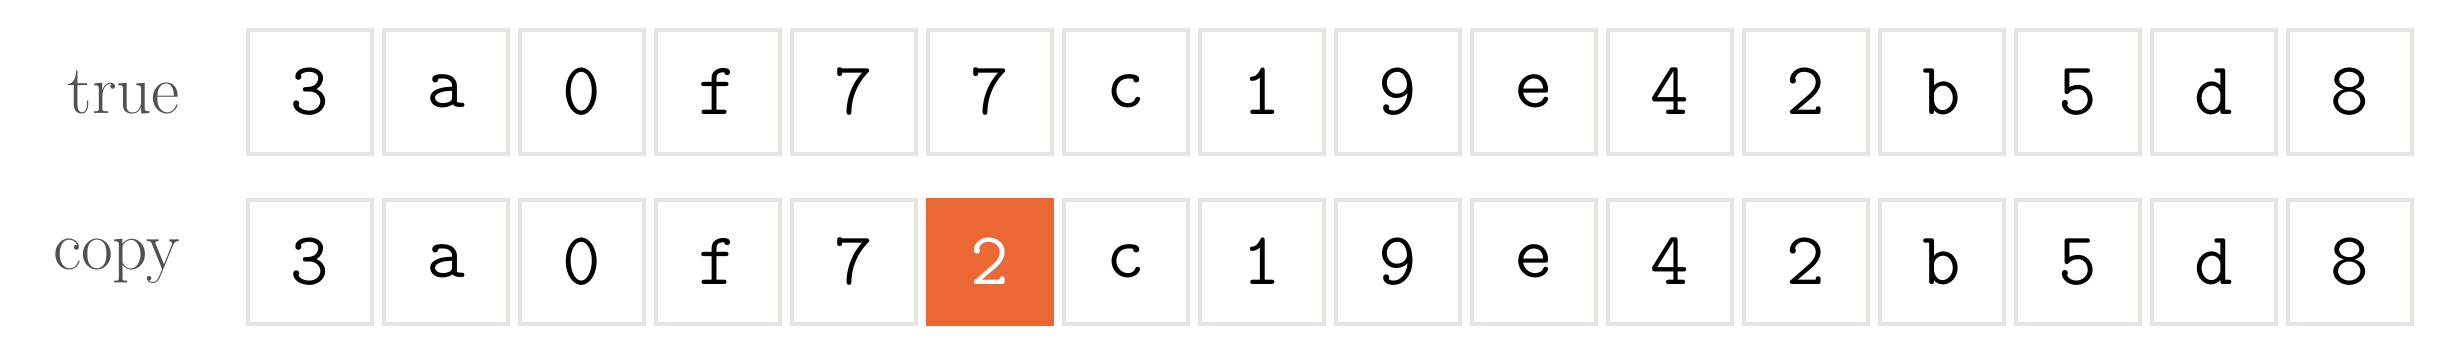
\begin{tikzpicture}[node distance=0.06in]
    \foreach \t [count=\i] in {3,a,0,f,7,7,c,1,9,e,4,2,b,5,d,8} {
      \node[tok] (s\i) at (\i*0.68in,0) {\t};}
    \foreach \t [count=\i] in {3,a,0,f,7,2,c,1,9,e,4,2,b,5,d,8} {
      \ifnum\i=6 \node[bad] (c\i) at (\i*0.68in,-0.85in) {\t};
      \else \node[tok] (c\i) at (\i*0.68in,-0.85in) {\t};\fi}
    \node[left=0.2in of s1,font=\small,text=ink2,anchor=east] {true};
    \node[left=0.2in of c1,font=\small,text=ink2,anchor=east] {copy};
  \end{tikzpicture}
  \par\raggedright\vspace{0.25in}
  \textbf{Task.} Score the true sequence and its 8 copies.\\
  \textbf{acc9}: true one ranked first (chance $1/9$).
  \textbf{pairwise}: true beats one copy (chance $1/2$).

  \vspace{0.15in}
  \textbf{Capacity, in theory.} Recall needs all $4N$ bits (1{,}024 at $N{=}256$).
  Recognition needs a few: keeping only the token sum mod 16 (4 bits) gives acc9 0.85;
  adding a position-weighted sum (8 bits) gives 0.965, at \emph{every} $N$.
\end{block}
%----------------------------------------------------------------- model
\begin{block}{Model: one network, two readouts}
  2-layer Gated DeltaNet-2 (\texttt{fla}), width 128, one head.
  The only memory is the recurrent state, $d_k{\times}d_v$ per layer: $128{\times}128$ (16{,}384 numbers) down to $16{\times}4$ (64).

  \vspace{0.2in}\centering
  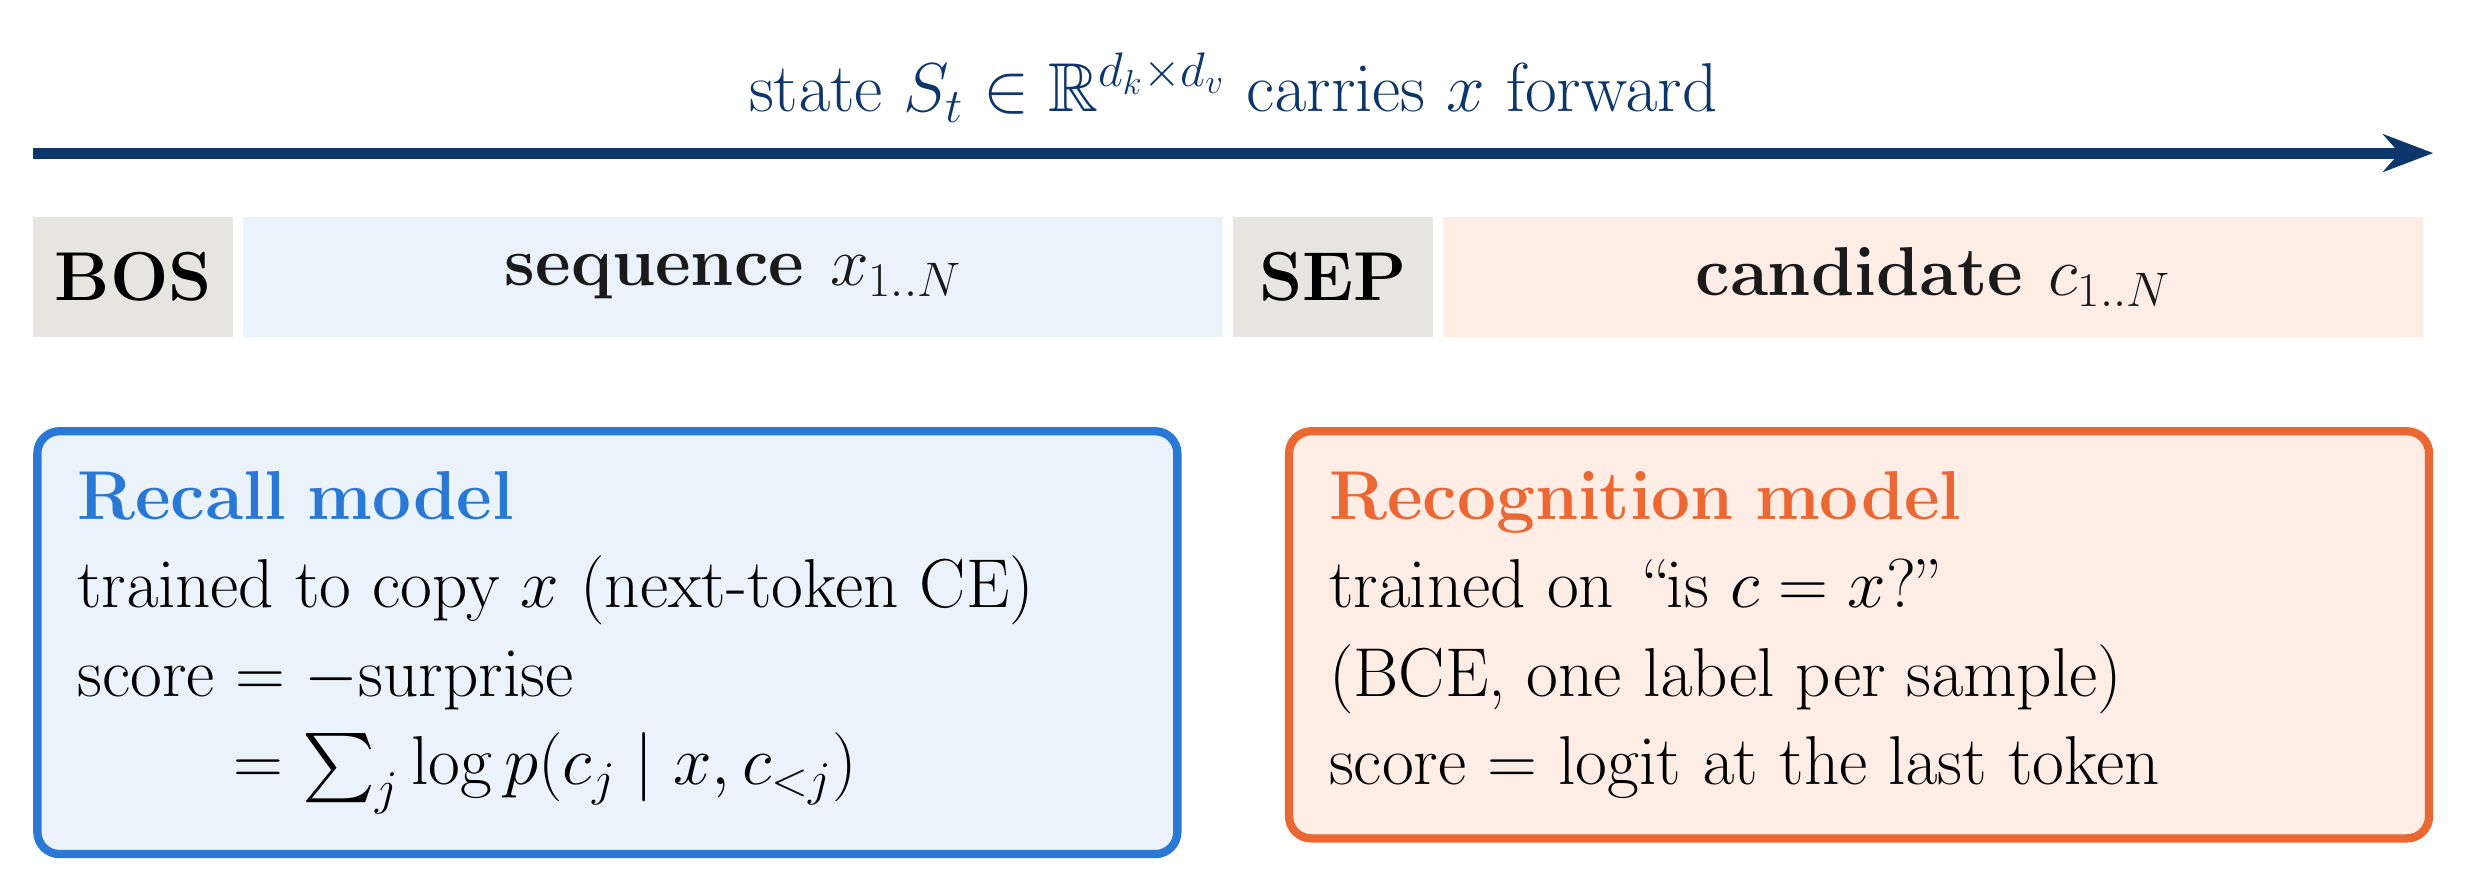
\begin{tikzpicture}[x=1in,y=1in]
    \tikzset{cell/.style={draw=none,minimum height=0.6in,inner sep=0pt,font=\small\bfseries}}
    \node[cell,fill=rule,minimum width=1.0in] (b) at (0.5,0) {BOS};
    \node[cell,fill=recallbg,minimum width=4.9in,text=ink] (s) at (3.5,0) {sequence $x_{1..N}$};
    \node[cell,fill=rule,minimum width=1.0in] (p) at (6.5,0) {SEP};
    \node[cell,fill=recogbg,minimum width=4.9in,text=ink] (c) at (9.5,0) {candidate $c_{1..N}$};
    \draw[-{Stealth[length=0.25in]},line width=4pt,navy] (0,0.62) -- node[above,font=\small,text=navy]
      {state $S_t\in\mathbb{R}^{d_k\times d_v}$ carries $x$ forward} (12.0,0.62);
    % readouts
    \node[draw=recall,line width=3pt,fill=recallbg,rounded corners=8pt,text width=5.3in,align=left,
      inner sep=0.2in,anchor=north west,font=\small] (lm) at (0.0,-0.75)
      {\textcolor{recall}{\bfseries Recall model}\\ trained to copy $x$ (next-token CE)\\
       score $=-$surprise\\ $\phantom{\text{score}}=\sum_j\log p(c_j\mid x,c_{<j})$};
    \node[draw=recog,line width=3pt,fill=recogbg,rounded corners=8pt,text width=5.3in,align=left,
      inner sep=0.2in,anchor=north east,font=\small] (cl) at (12.0,-0.75)
      {\textcolor{recog}{\bfseries Recognition model}\\ trained on ``is $c=x$?''\\ (BCE, one label per sample)\\
       score $=$ logit at the last token};
  \end{tikzpicture}
\end{block}\vspace{-0.55in}
\end{minipage}\hfill
%======================================================================= column 2
\begin{minipage}[t]{15.3in}\vspace{0pt}
\begin{block}{\textcolor{recall}{1}\enspace Full-size state: recall is easy, the classifier never starts}
  At $128{\times}128$ the \RC{recall model} copies every length almost perfectly (exact copy $0.988$ at $N{=}256$),
  and its surprise ranks the true sequence first in \emph{every} test sample.
  The \RG{recognition classifier} fails from $N{=}64$ on.

  \vspace{0.2in}
  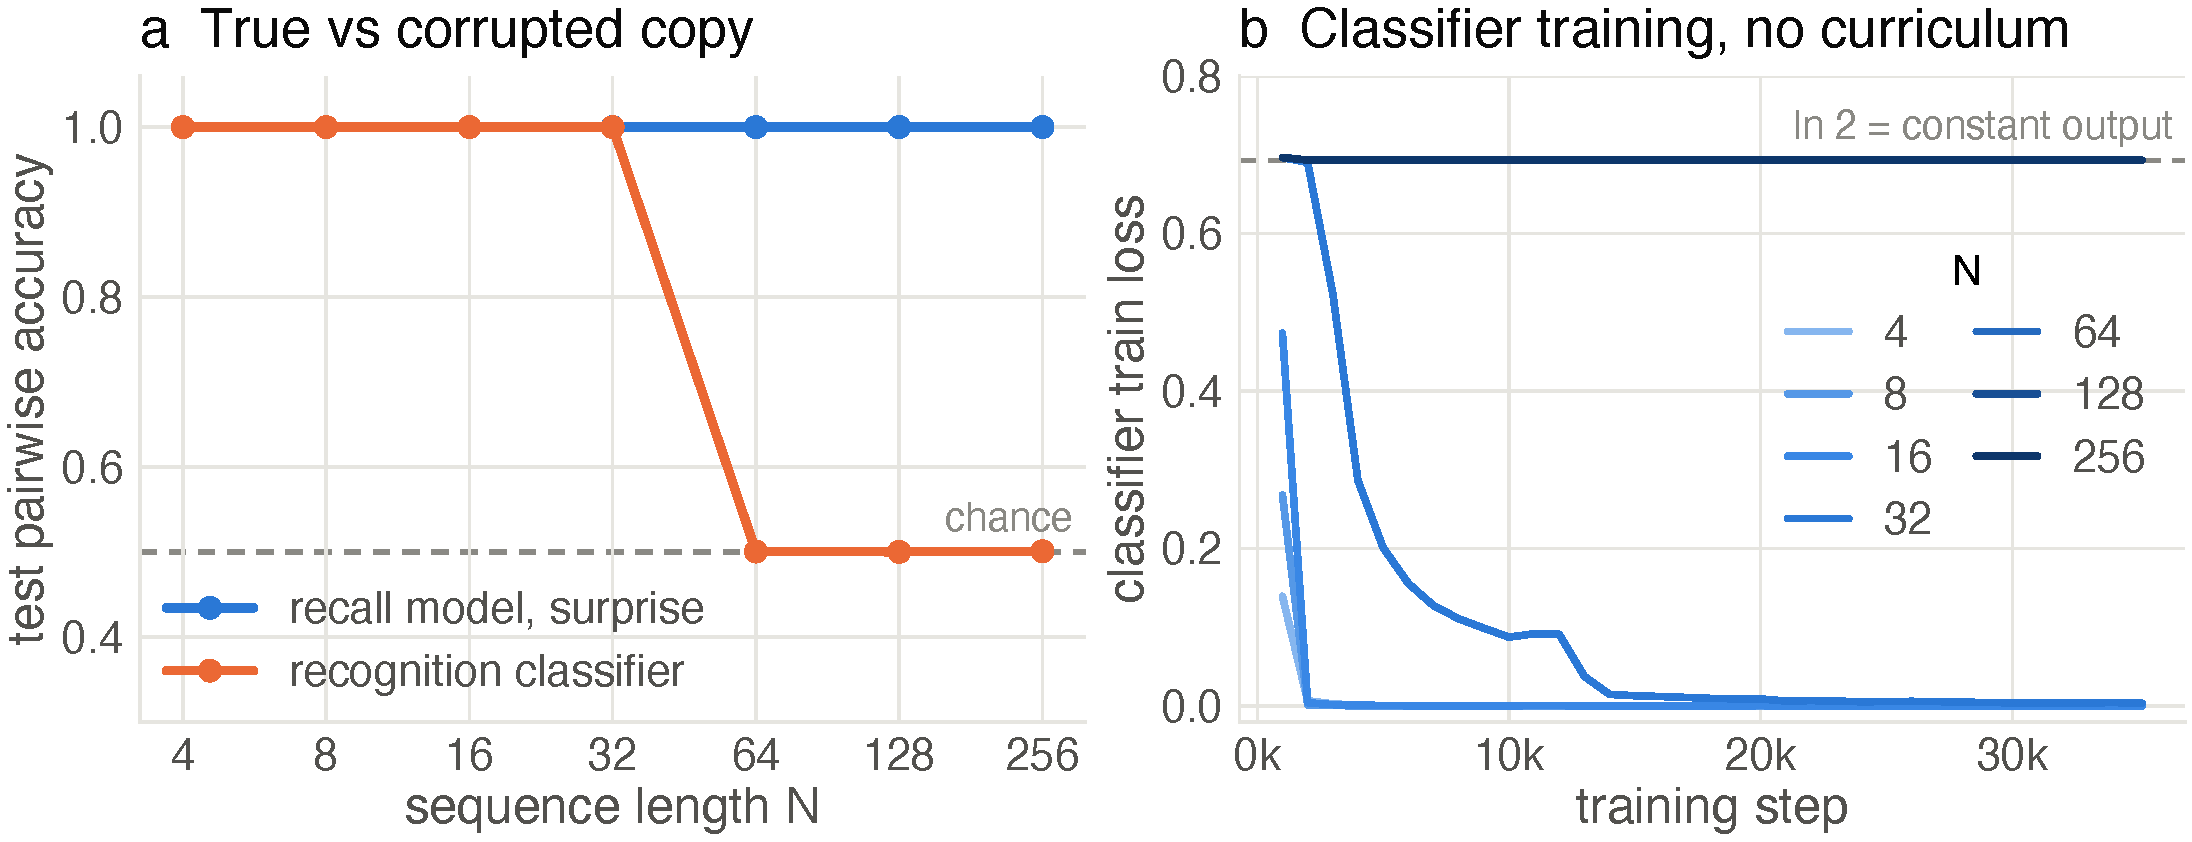
\includegraphics[width=\linewidth]{full_state.pdf}
  \figcap{Test on 100k sequences, 10 epochs, seed 0. (b) Classifier BCE, mean over 1{,}000 steps, one line per $N$.}
  \begin{itemize}
    \item The loss sits at $\ln 2$ for all 35k steps: a constant output, gradients decay to ${\approx}0.03$.
    \item Same network learns recall in ${<}1{,}000$ steps $\Rightarrow$ an \textbf{optimisation} failure,
          not a capacity limit. One label per sample says little about 2 differing tokens out of 256.
  \end{itemize}
\end{block}

\begin{block}{\textcolor{curr}{2}\enspace A length curriculum lets the classifier learn}
  For the first half of training, train on prefixes $16, 32, \ldots, N$ (equal time each),
  with easy, heavily corrupted negatives fading out.
  Then switch to full length and the benchmark's copies.

  \vspace{0.2in}
  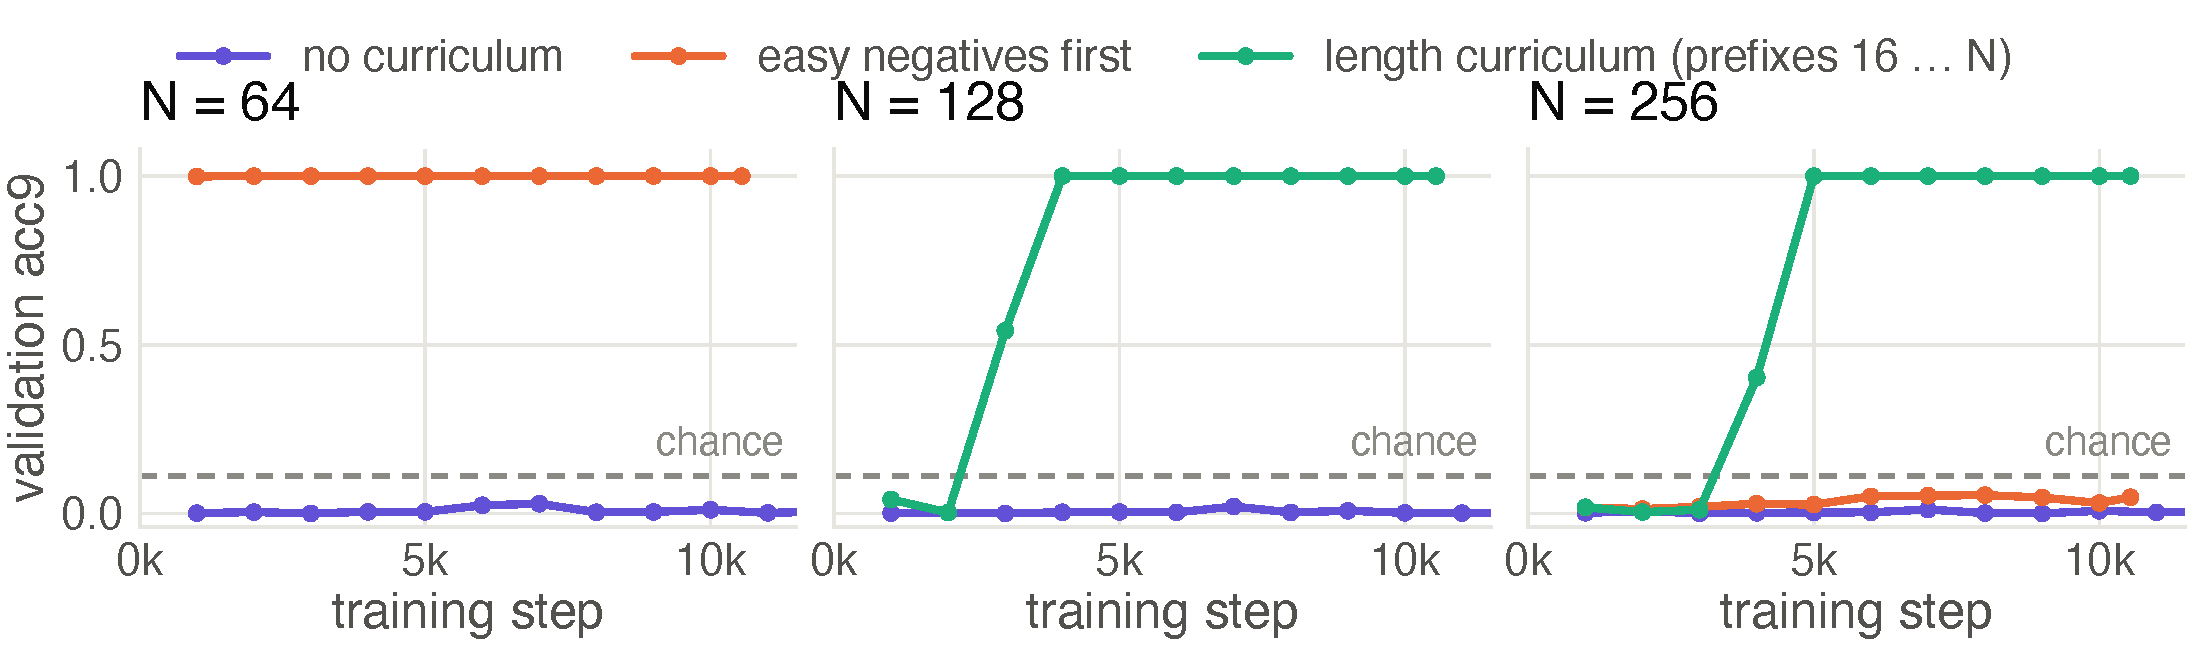
\includegraphics[width=\linewidth]{curriculum.pdf}
  \figcap{Validation acc9 (full-length sequences) of the $128{\times}128$ classifier. Curriculum runs: 3 epochs; no-curriculum runs: 10 epochs (first 11k steps shown).}
  \begin{itemize}
    \item \textcolor{curr}{\textbf{Length curriculum}}: acc9 $=1.000$ at $N{=}128$ and $256$.
    \item Easy negatives alone fix $N{=}64$ but \textbf{not} $N{=}256$.
    \item Comparing learned on short prefixes carries over to long ones.
    \item In the sweep, \textbf{all 42} curriculum-trained classifiers learn; none ends at $\ln 2$.
  \end{itemize}
\end{block}\vspace{-0.55in}
\end{minipage}\hfill
%======================================================================= column 3
\begin{minipage}[t]{15.3in}\vspace{0pt}
\begin{block}[colframe=navy,boxrule=5pt]{\textcolor{recog}{3}\enspace Shrinking the state: recall goes first}
  6 state sizes ($16{\times}4$ to $128{\times}128$) $\times$ 7 lengths $\times$ 2 objectives: 84 runs, 10 epochs each,
  tested on 100k sequences.

  \vspace{0.2in}
  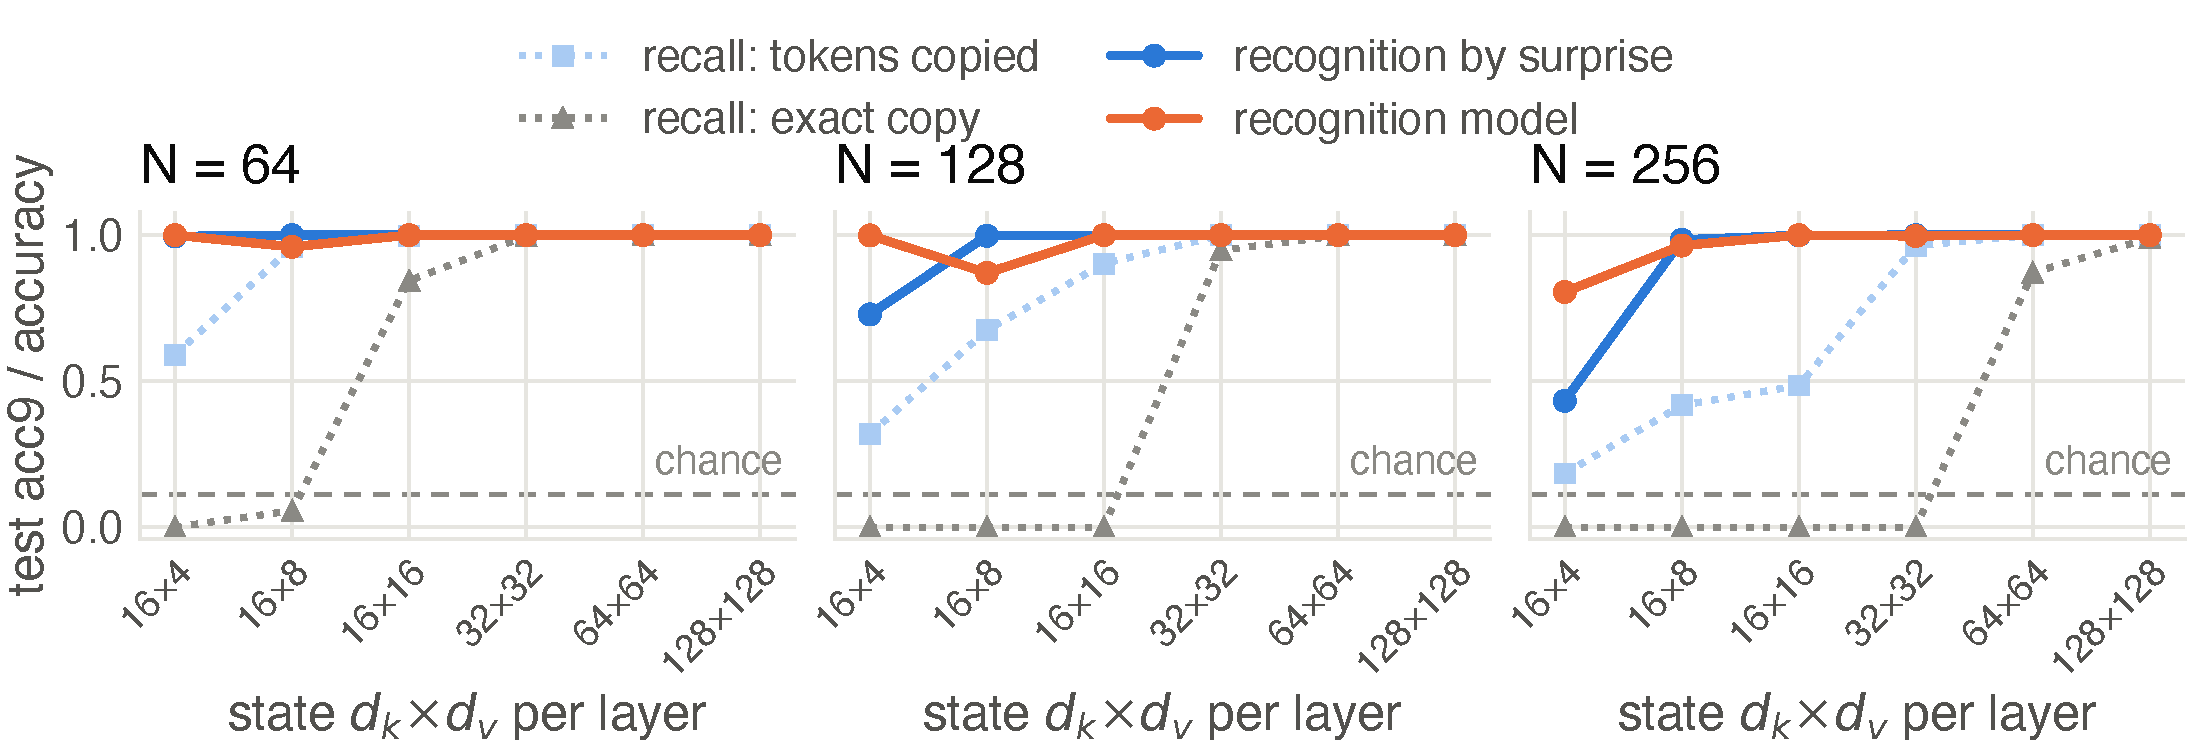
\includegraphics[width=\linewidth]{sweep.pdf}
  \figcap{Test acc9: \RC{recall model's surprise}, \RG{recognition classifier}. Dotted: recall. $N\le32$: all ${\ge}0.87$.}

  \vspace{0.1in}
  \begin{itemize}
    \item \textbf{Recognition outlasts recall.} At $16{\times}16$, $N{=}256$ the recall model keeps ${\sim}$half the bits
          (${\ge}536$ of 1{,}024) and copies no sequence exactly, yet both readouts score acc9 ${\ge}0.999$.
          Surprise reaches 0.98--1.00 while ${\ge}\tfrac13$ of the bits are kept: above the 8-bit checksum.
    \item \textbf{Smallest state: the classifier wins.} \\
          \begin{tabular}{@{}lccc@{}}
            $16{\times}4$ & recall tokens & \RC{surprise} acc9 & \RG{classifier} acc9 \\ \midrule
            $N{=}128$ & 0.32 & 0.73 & \textbf{1.00} \\
            $N{=}256$ & 0.18 & 0.43 & \textbf{0.81} \\
          \end{tabular}\\[0.15em]
          Still below a 4-bit checksum (0.85): far from the best code the state could hold.
    \item At $16{\times}8$ surprise is as good or better ($N{=}128$: 1.00 vs.\ 0.87).
  \end{itemize}

  \vspace{0.2in}
  \RG{The $16{\times}4$ classifier} at $N{=}256$ learns only once the curriculum reaches full-length prefixes:
  \par\vspace{0.1in}
  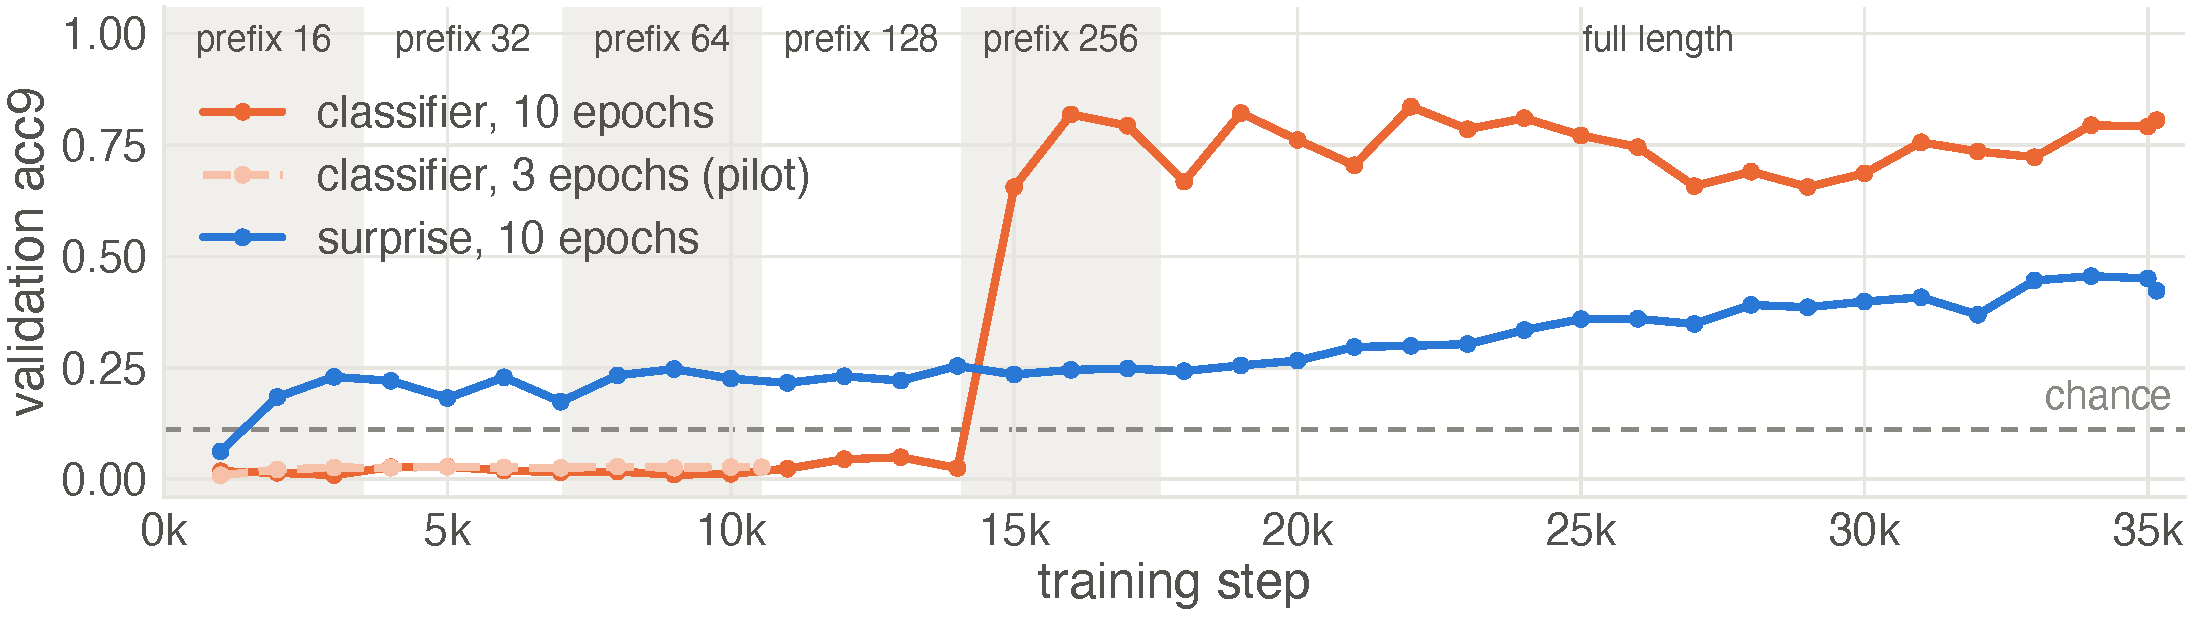
\includegraphics[width=\linewidth]{small_state_curves.pdf}
  \figcap{Validation acc9, $16{\times}4$, $N{=}256$; shading: curriculum stages. The 3-epoch pilot never left $\ln 2$.}
\end{block}

\begin{block}{Next}
  \begin{itemize}
    \item \textbf{Seeds 1--2} at the three smallest states (60 runs): is the $16{\times}4$ win real, and the $16{\times}8$ dips noise?
    \item \textbf{Longer curriculum} at small states: those runs were still improving.
    \item \textbf{Harder benchmarks} where checksums fail; $K$ stored sequences per context.
  \end{itemize}
  \vspace{0.1in}
  {\footnotesize\color{ink2} Seed 0 only. The three smallest states shrink $d_v$ only (fla kernels need $d_k\ge16$);
   across $16{\times}4$--$16{\times}16$ the parameter count changes by 4\%.\par}
\end{block}\vspace{-0.55in}
\end{minipage}
\end{document}
